
\documentclass[12pt, oneside]{article}   	% use "amsart" instead of "article" for AMSLaTeX format
%\usepackage{geometry}                		% See geometry.pdf to learn the layout options. There are lots.
%\geometry{letterpaper}                   		% ... or a4paper or a5paper or ... 
%\geometry{landscape}                		% Activate for rotated page geometry
%\usepackage[parfill]{parskip}    		% Activate to begin paragraphs with an empty line rather than an indent
\usepackage{graphicx}				% Use pdf, png, jpg, or eps§ with pdflatex; use eps in DVI mode
								% TeX will automatically convert eps --> pdf in pdflatex		
\usepackage{amssymb}
\usepackage{amsmath}
\usepackage{amsfonts}
\usepackage{amssymb}
\usepackage{graphicx}
\usepackage{listings}
\usepackage{hyperref}
\usepackage[left=1.00in, right=1.00in, top=1.00in, bottom=1.00in]{geometry}
%SetFonts

%SetFonts


\title{Crafting a Compiler}
\author{Nevin Leh\\Aaron Newhall\\Tim Weghen}
%\date{}							% Activate to display a given date or no date

\begin{document}
\begin{titlepage}
	\maketitle
\end{titlepage}
\setcounter{page}{2}
\tableofcontents
\section{Introduction}
The purpose of this project is to create a compiler. This is essentially a translation of a human readable language into a computer 
readable language. This is being done to explore the realm of computing at the most basic level and to illustrate the process of 
creating a compiler from start to finish.

When completing a degree in nearly any field it is necessary to complete a
course known as a capstone course. In this course, especially in fields such as
engineering, undergraduates get in groups and work on a project that lasts an
entire semester. The idea of these projects is basically a culmination of as many
of the main topics a student has learned in route to completing their degree as
possible. In computer science there are not many ideal projects that could be
chosen to highlight everything a CS student learns during their studies. However,
the one that was chosen for Montana State University computer science students
was to get into groups and create a Compiler. This project serves as a great
opportunity to not only show the department what their graduates are learning,
but it also serves to show the graduates themselves what they are capable of.
This idea of can roughly be thought of as a motivation for the project and class as
a whole

The object of this project was to create a compiler that was based on a
language created by the instructor. In this case the language given was called
“Tiny”. This language was a fairly simple language created so that creating a
compiler that worked for it would take the right amount of time. If the language
were too complicated the project would have been much too difficult to complete
in the given amount of time. The students were given the language and small test
programs, the compiler would then be designed to take in these programs in their
raw form, exactly as a programmer would have written them, break them down
into an intermediate language, then finally output a form broken down into a basic
machine language so the computer could actually perform the intended function
of the given code. Through lots of hard work and time spent, our group has
succeeded in creating a functioning compiler for the language Tiny that was
given to us.

This project was separated into four main steps each step building upon
the last in order to get us closer to the ultimate goal, these steps included:
Scanner, Parser, Symbol Table, and Semantic Routines. Each of these steps
was accompanied by not only hours and hours of class time learning the theories
and application behind each, but also mandatory labs created by the instructor to
give us hands on experience with the ideas behind the given step. This Report
will serve as a walk through of the entire process of creating a functioning
compiler. First, compilers in general will be explained including a brief history of
compilers with some basic information. This information will detail what exactly a
compiler does, meaning what is its purpose, along with a more technical look into
the different parts and where they fit in and what they actually do. Also, included
will be some information on real world example of compilers.

Next, the report will go into great detail of the process that our individual
group went through during each step of the project. In each section the process
of the given step is discussed including the method we used and how we
implemented the given step, as well as the many difficulties we encountered
along the way and how we got passed them. Also, the compiler as a whole will
be looked at including the process as a whole including tools used and how we
combined all the parts to create the final product. The final section of the report
will be a conclusion that details how the final product could be improved upon
given more time and resources. These improvements will be presented as a plan
and will cover topics such as optimization, including run-time memory
management as well as code optimizations. However, In order to fully understand
this project, as well as how it could be improved upon, and what exactly the
purpose of this capstone project is, one must learn what exactly a compiler is.
\section{Background}
Long before the modern era of programming languages programming was
much different. Instead of writing elaborate programs using development
environments with built in tools and libraries programmers had to
write code in languages such as assembly which is essentially machine code.
This style coding was much less efficient than writing programs in a high-level
language, which could be reused on different systems. However, early compilers
didn't always function better than hand written assembly and way many times
hindered by the lack of system memory.

The term compiler actually existed years before a complete compiler was
even created, though it wasn’t widely used, allegedly given the name by well
known computer scientist Grace Hopper while working on the A-O System
language. The “compiler” she was using was far from what comes to mind when
talking about compilers in the modern era. During the 50’s there were many other
scientists toying with the idea of compilers, but it wasn’t until 1957 that the first
complete compiler was born, created at IBM by the FORTRAN team lead by
John Backus. Work on compilers throughout the ‘60s paved the way for many of
ideas essential to our modern compilers. Early compilers were written mostly in
assembly, but by the 70’s compilers for languages such as C or Pascal were
written in their own languages. In the current era there are almost too many
different compilers to count. Each programming language has several, and more
and more are being created all the time.

So, what is a compiler? In a very general sense, a compiler is a computer
program that translates a computer program written in a given language, called a
source language, into an equivalent program of a different language, this
language is usually referred to as the target or output language. Though this may
seem like a pointless act, it actually serves a purpose. A compiler typically takes
a program written in a high level programming language (such as Java, C++,
Python, etc) and breaks it down into a form know as object code or machine code
that can be easily executed by a computer of virtual machine. Though compiling
from a high level language to a low level language isn’t always the case, it is
the most likely case. There are also compilers made to change one high level
language into another high-level language or even a low level language to a high
level. Though there may be many different kinds of compilers, one thing is for
sure, any programs written in a high-level programming language must be
translated to object code before it can be executed.

Most modern compilers are laid out in a similar way, meaning they have
the same basic parts and function in a similar way. Due to system restrictions
early compilers were divided in to multiple passes, each pass being a “run”
through the source code, gradually building up the internal data in the compiler.
Modern compilers like the one being created for this assignment work in two
stages, a front-end and a back-end. The front-end translates the code into an
intermediate representation, and the back-end produces the output language.
This project split up the process into four main steps: the Scanner, Parser,
Symbol Table, and Semantic Routines. Each of these steps play a pivotal role in
the compiler and without and one of them the process would not be possible. The
first step of the process when a written program comes in contact with the
compiler is the scanner, sometimes referred to a tokenizer or lexical analysis.
The Scanners is responsible for break up the input stream of the source code
into individual tokens or terminals, identifying the token type, and passing tokens
one at a time to the next in the process. These tokens are defined by the creator
of the compiler and can include items such as keywords, identifiers, or symbol
names. The scanner can be compared to the dictionary in human language in that it keeps the list of tokens(words) and their syntax(token type).

The next step in the process is called the parser. The parser contains
rules of the given language, and it is in this step that many syntax
errors are caught. These rules are usually referred to as a grammar. The parser focuses on the structure of the program identifying
the order of the tokens using a structure called a parse tree or abstract syntax
tree. The parser combined with the scanner make up the front-end portion of the
compiler.

\begin{figure}[h!]
	\centerline{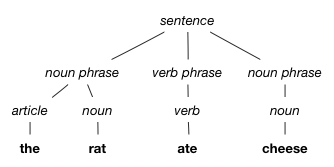
\includegraphics[width=.4\linewidth]{pics/p_tree}}
	\caption{Parse tree for an English sentence}
\end{figure}

 The third step of the process has to do with what is referred to as the
symbol table. The symbol table is an important step in the process because it is
actually a data structure created and altered by the compiler in order to store
information about the occurrences of items such as variable names and their
declarations as well as scope. The symbol table stores the names of all the
entities in a structured form to be used in the last step of the compiler.

The final step of the compiler can be referred to as the Semantic
routines. It is during this step that the main function of the compiler is completed.
During this step the compiler uses the symbol table generated by the front-end of
the compiler and generates an intermediate representation of the high-level
language program that went in. The compiler then translates that IR code into its
last step of compilation, which is the low level machine code ready to be
executed by the computer or virtual machine.

\begin{figure}[h!]
	\centerline{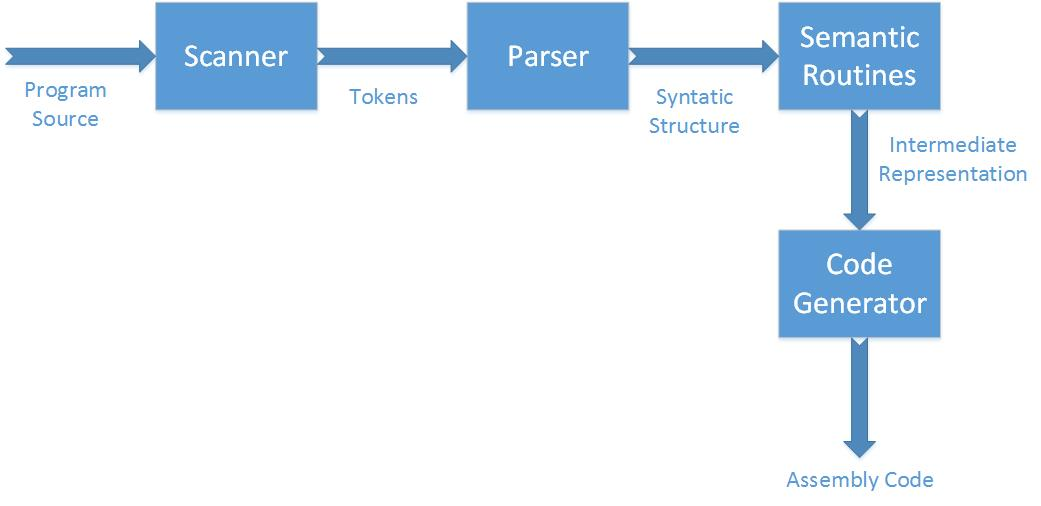
\includegraphics[width=.4\linewidth]{pics/diagram}}
	\caption{Components of the typical compiler}
\end{figure}


\section{Methods and Discussion}
\subsection{Scanner}
\subsubsection{Tools}
The lexer tool lex, provided by the PLY package for python, was used to create the scanner. This tool was chosen for it's simplicity and ease of use in creating a scanner. It is very similar to the lex program provided with most unix/linux systems and has a relatively easy setup compared to other scanner generators such as ANTLR. 
Initially ANTLR was the chosen scanner, but the very specific dependencies proved to be too complicated and a switch to PLY was decided upon. 

\subsubsection{Implementation}
Implementing the scanner with the help of PLY is a pretty trivial process. The guide
provided by the creators of PLY proved to be invaluable and very effective at
introducing the basics of creating a scanner. First, all of the token types have to be defined at the start of the scanner as a
list. These token types are used to define different types of valid tokens. These token types are necessary because the parser in the next step needs to be able to assemble the tokens into a parse tree. For the micro  grammar the token types IDENTIFIER, FLOATLITERAL, STRINGLITERAL, COMMENT, KEYWORD, and OPERATOR were defined.

The second step was to define regular expressions that match tokens to their token types. Regular expressions are used to define patterns within strings and have numerous uses. Each token type has a regular expression that defines the strings that need to match with that token type. The scanner then takes a Micro program as input and constantly takes
the first matching token and saves that token value along with its type in a list. If a part of the string doesn't get matched with a token type there is an error and the scanner stops and lets the user know that an invalid token has been
matched. If the list doesn't have any errors it will be passed to the parser to have the grammar of the program analyzed. 

The following code shows a very simple implementation of scanner that has one token type KEYWORD that matches the strings "START" and "END .
\begin{lstlisting}
	tokens = ('KEYWORD')
	t_KEYWORD = (r"BEGIN|END")
\end{lstlisting}
The syntax of defining tokens is very important as the PLY package uses the syntax to make a program that takes the program as input and returns a list of tokens and token types.

For the most part the rest of the leg work for creating the list of tokens is handled internally be the lexer.py file provided by PLY. One exception to this is that the scanner needs to ignore certain characters and lines such as spaces, tabs, and comments. To do this another token rule must be defined that starts with t\_ignore. The scanner will then match these like a regular token but omit them from the final token list provided to the parser. This ensures that an unintended error doesn't happen.

\subsubsection{Difficulties}
For the most part implementing the scanner went off without a hitch. However, there were several aspects of creating the regular expressions and the order in which these regular expressions were executed that created some difficulties. For example, "ENDWHILE" will be matched by the rule 
that defines "END". To get around this a lookahead was used so "END" would only match if it wasn't followed by "WHILE". Another way to do this would be to put "ENDWHILE" before "WHILE" in the regular expression but it was decided that the lookahead was more robust and easier to read. The following lines of code  shows a regular expression that will match "END" but not "ENDWHILE".
\begin{lstlisting}
	(r"END(?!WHILE)")
\end{lstlisting}

Another tricky part was finding a way of excluding the comments from the output file. It was finally determined that a prefix of t\_error was needed to ignore the comments within the parser. This took a while as it was not realized that PLY would accept multiple t\_error rules and it had already been used to ignore whitespace.
 
This scanner had to be modified multiple times to make it work better with the parser. The changes that were applied
will be discussed in full there but in general the scanner was not specific enough and needed more token types to effectively check that the program had correct grammar.
		
		
		
\subsection{Parser}
\subsubsection{Tools}
The parser tool yacc, provided with PLY, was used to create the parser because PLY was used to make the scanner. This was important because yacc is designed to take the output from lex as input. Once again this helped streamline the process of creating a functional compiler.
The guide provided with ply was used to create the bare bones of the code.

\subsubsection{Implementation}
Implementing the parser with the help of yacc was a pretty strait forward task. Luckily the grammar for Micro was provided in a file and  for the most part these rules
could be copy and pasted into yacc with the correct syntax. The following lines of code from the parser illustrate how a rule is defined in yacc.
\begin{lstlisting}
def p_assign_expr(p):
    'assign_expr : id EQ_EQ expr'
\end{lstlisting}

While most of the grammar rules could be copy and pasted, some rules had to have some work done on them
to make them work with our scanners output. The most obvious were the operators. In the grammar file the operators were the literal operators such as + or *. To make these work changes the operators were given names such as PLUS or
MINUS. To check if an input program is valid the parser calls the scanner and gets the token list from it. It then
has yacc parse through the tokens and verifies that the program is grammatically correct.
\begin{figure}[h!]
	\centerline{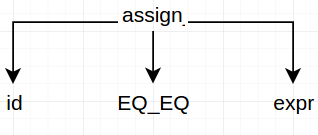
\includegraphics[width=.4\linewidth]{pics/parse_tree}}
	\caption{Parse tree of above rule}
\end{figure}

\subsubsection{Difficulties}
One of the main difficulties that was encountered was the fact that the initial scanner that was
made did not match all the tokens the grammar needed. Initially, keywords and operators were matched as
KEYWORD and OPERATOR. For the parser more specific token recognition was needed such
as differentiating a comma from a semi colon. To fix this each operator got its own token and regular expression. In addition all the keywords were were broken out and added to the token list individually.

 Another difficulty was the fact that the parser would assume a keyword was an
identifier since the identifier rule in the scanner had higher precedence than the keyword one. This is because in yacc the shortest rule is used first. To fix this a function rule was added for identifiers. A function rule is unique in that conditions other than regular expressions can be used to decide whether the token matches. In this case an extra condition that dictated that an identifier cannot match a keyword was added to fix this problem.

In addition there was a problem with mixed syntax from several examples which were impossible to figure out for the longest time. Finally it was found that some rules in the scanner started with a
capital T instead of a lower case t. It turned out that they all had to start with a lowercase t or they all had to start with an uppercase one.
\subsection{Symbol Table}
\subsubsection{Theory}
The implementation of the symbol table is unique in that an external tool such as PLY are not used. In addition the symbol table actively interacts with the parser in that the parser calls the symbol table to add variables and scopes. The symbol table is essentially a stack of of python dictionaries with each dictionary representing a different scope. The first scope on the stack is the global scope and is available from every other scope. As functions are called new scopes are pushed onto the stack and as functions return the top scope is popped of. As variables are declared they are added to the current scopes dictionary. If a value is already in the current scope or the global scope it is an illegal declaration and an error results.

In addition there are special scopes called blocks. These result in a new scope being added to the stack when an if or loop statement is called. These scopes are unique in that variables declared in the block cannot be in the most recent function scope or the global scope. These scopes are popped off the stack when the block ends so they cannot be used after the loop or if statement ends.
\subsubsection{Implementation}
While the symbol table seems pretty straightforward in theory, in practice it proved much more difficult. The symbol table was designed as a separate python class that contains a stack of python dictionaries and various methods for adding variables and scopes to the stack correctly. An instance of this class was created in the parser and, as the rules that corresponded to adding scopes or variables were executed, the corresponding methods were called to manipulate the stack in the correct way. 

To do this the tokens had to be percolated up through the grammar. Though the exact details of how yacc does this were never fully understood, a functional solution was found.  The functions that define the grammar take in an input P. This P corresponds to the grammar rules that make up that grammar rule. To better illustrate this reference this grammar function.
\begin{lstlisting}
def p_id_list(p):
	'id_list : id id_tail'
	p[0] = [p[1]] + p[2]
	
def p_id(p):
	'id : IDENTIFIER'
	p[0] = p[1]
\end{lstlisting}
It can be seen that p\_id takes in p where p is a list. p[0] is the value that will be percolated up through the grammar and corresponds to the left side of the grammar rules. The rest of the slots in the list correspond to what rules make up this rule. So in this case by making p[0] = to p[1], when this id is used its value will be the value of the token IDENTIFIER. In addition if that id is used by p\_id\_list the slot p[1] will be will now have the value of the IDENTIFIER. 

If p\_id\_list is in another grammar rule, it will be composed of its id and id\_tail in a list. In this way the values that need to be added to the symbol table can be added when the scopes are declared such as in an if statement. 
\begin{lstlisting}
def p_if_stmt(p):
	'if_stmt : s_if L_PAR cond R_PAR decl stmt_list else_part ENDIF'
	table.block_end()
\end{lstlisting}
	Here it can be seen that if rules are passed up in this way the variables that are being declared can be accessed by checking p[5] for the variables that need to be added to the scope of the block.


\subsubsection{Difficulties}
One of the main difficulties was figuring out where to call functions from the symbol table class in the parser. Since the parser is an LR-parser the functions in the parser are actually called in reverse. So an IDENTIFIER is set to an id before it is known what it is for. This meant that the scope starts and stops were in reverse order. For example, an if grammar function will execute before the grammar function that defines a function will execute. To remedy this some new grammar rules were added. Here is one.

\begin{lstlisting}
def p_s_if(p):
	's_if : IF'
	table.block_start()
\end{lstlisting}
	Here the token IF was taken out of the p\_if\_stmnt and placed in a new rule. Since this rule is a level below the if rule it executes before the variables are declared for it. This calls the block\_start function of the symbol table which adds a scope to the stack before variables are declared.
	
	\begin{figure}[h!]
		\centerline{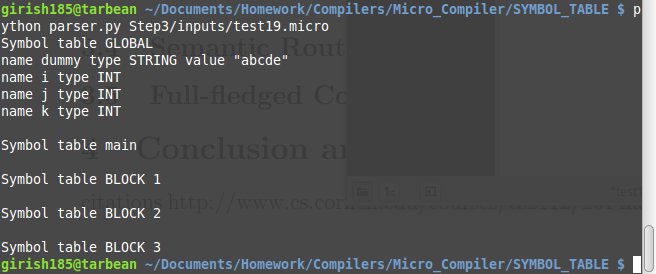
\includegraphics[width=.4\linewidth]{pics/sybol_output}}
		\caption{sample output of symbol table}
	\end{figure}
	
\subsection{Semantic Routines}
The semantic routines part of a compiler consists of two parts.

\subsection{Full-fledged Compiler}

\section{Conclusion and Future Work}

citations
http://www.cs.cornell.edu/courses/cs2112/2014fa/lectures/lecture.html?id=parsing



\end{document}  